\documentclass[12pt, a4paper]{article}

\usepackage{algorithm, algorithmic, amsmath, amsfonts, amssymb, amstext, amscd, amsthm, bbm, CJKutf8, color, dsfont, enumerate, float, graphicx, hyperref, lipsum, makeidx, mathrsfs, mathtools, marvosym, soul, stmaryrd, url, verbatim, xcolor, xfrac}
\usepackage[left=2cm,top=2cm,right=2cm,bottom=2cm,bindingoffset=0cm]{geometry}
\hypersetup{
    colorlinks=true,
    linkcolor=black!50!red,
    urlcolor=black!50!red
}
\allowdisplaybreaks

\newenvironment{subproof}[1][Proof]
    {\proof[#1]\leftskip=1cm\rightskip=1cm}
    {\endproof}

%theorems with custom numbering
%\newtheorem{innerthm}{Theorem}
%\newenvironment{thm}[1]
    %{\renewcommand\theinnerthm{#1}\innercustomthm}
    %{\endinnerthm}

\newtheorem{theorem}{Theorem}
\newtheorem{lemma}{Lemma}
\newtheorem{proposition}{Proposition}
\newtheorem{corollary}{Corollary}
\newtheorem{claim}{Claim}
\newtheorem{conjecture}{Conjecture}
\newtheorem{justification}{Justification}
\newtheorem{definition}{Definition}
\newtheorem*{remark}{Remark}
\newtheorem*{note}{Note}

\renewcommand{\restriction}[1]{\downharpoonright_{#1}}
\renewcommand{\qedsymbol}{QED}
\renewcommand{\leq}{\leqslant}
\renewcommand{\geq}{\geqslant}
\renewcommand{\and}{~\wedge~}
\newcommand{\defn}{\coloneqq}
\newcommand{\disj}{~\vee~}
\newcommand{\xor}{~\oplus~}
\newcommand{\divides}{~|~}
\newcommand{\given}{\middle|}
\newcommand{\suchthat}{~\middle|~}
\newcommand{\contradiction}{~\text{\Large \Lightning}}
\newcommand{\conj}[1]{\overline{#1}}
\newcommand{\mean}[1]{\overline{#1}}
\newcommand{\integral}[1]{\smashoperator{\int_{#1}}}
\newcommand*\diff{\mathop{}\!\mathrm{d}}
\newcommand{\E}[1]{\mathbb{E}\sqparens*{#1}}
\newcommand{\Esub}[2]{\mathbb{E}_{#1}\sqparens*{#2}}
\newcommand{\var}[1]{\mathrm{Var}\parens*{#1}}
\newcommand{\cov}[2]{\mathrm{Cov}\parens*{#1, #2}}
\newcommand{\der}[2]{\frac{\diff{#1}}{\diff{#2}}}
\newcommand{\dern}[3]{\frac{\diff^{#3}{#1}}{\diff{#2}^{#3}}}
\newcommand{\derm}[3]{\frac{\diff^{#3}{#1}}{\diff{#2}}}
\newcommand{\prt}[2]{\frac{\partial{#1}}{\partial{#2}}}
\newcommand{\prtn}[3]{\frac{\partial^{#3}{#1}}{\partial{#2}^{#3}}}
\newcommand{\prtm}[3]{\frac{\partial^{#3}{#1}}{\partial{#2}}}

\newcommand{\C}{\mathbb{C}}
\newcommand{\N}{\mathbb{N}}
\newcommand{\Q}{\mathbb{Q}}
\newcommand{\R}{\mathbb{R}}
\newcommand{\Z}{\mathbb{Z}}

\DeclareMathOperator{\lcm}{lcm}
\DeclareMathOperator*{\argmin}{arg\!\min}
\DeclareMathOperator*{\argmax}{arg\!\max}

\let\originalleft\left
\let\originalright\right
\renewcommand{\left}{\mathopen{}\mathclose\bgroup\originalleft}
\renewcommand{\right}{\aftergroup\egroup\originalright}
\newcommand{\zh}[1]{\begin{CJK}{UTF8}{gbsn}#1\end{CJK}}
\newcommand{\jp}[1]{\begin{CJK}{UTF8}{gbsn}#1\end{CJK}}

\DeclarePairedDelimiterX \inner[2]{\langle}{\rangle}{#1,#2}
\DeclarePairedDelimiterX \braket[2]{\langle}{\rangle}{#1 \delimsize\vert #2}
\DeclarePairedDelimiter \bra{\langle}{\rvert}
\DeclarePairedDelimiter \ket{\lvert}{\rangle}
\DeclarePairedDelimiter \abs{\lvert}{\rvert}
\DeclarePairedDelimiter \norm{\lVert}{\rVert}
\DeclarePairedDelimiter \set{\lbrace}{\rbrace}
\DeclarePairedDelimiter \seq{\langle}{\rangle}
\DeclarePairedDelimiter \parens{(}{)}
\DeclarePairedDelimiter \sqparens{[}{]}

\begin{document}

\title{Variance Reduction via Antithetic Sampling}
\author{Daniel Gonzalez\\{\small \it Department of Mathematics, Florida State University}}

\maketitle

\begin{abstract}
    Variational Bayesian inference methods are a family of techniques approximating intractable integrals, often employing stochastic optimization techniques.
    These methods typically use independent Monte Carlo samples to estimate gradients.
    In this paper, we give an overview of a technique employed in (\href{https://arxiv.org/pdf/1810.02555.pdf}{arXiv:1810.02555})
    for generating Normally-distributed Monte Carlo samples which are correlated, but more representative, and which can thus be used to reduce the variance in estimation.
\end{abstract}

\section{Introduction} \label{sec:1}
Gradient-based optimization methods are a robust and powerful way of attacking a wide class of problems in applied mathematics, science, and engineering.
Optimizing expectations using gradient optimization (e.g. gradient descent) is particularly prevalent in machine learning,
including variational inference and reinforcement learning.
Problems in these fields typically involve computing expectations and gradients which are analytically intractable.
Instead, practitioners frequently employ Monte Carlo methods to estimate those expectations and their gradients.
While Monte Carlo methods lead to unbiased estimation of the target expectations and gradients, they suffer from high variance when a small amount of samples are used.
The variance in a Monte Carlo estimator can be na\"ively  reduced by using more samples, but the computational cost quickly becomes impractical. 

One way of reducing the variance in the Monte Carlo estimators while maintaining a low number of samples is through the method of {\it antithetic variates}.
According to the antithetic variates approach, for every sample generated from a given distribution for the Monte Carlo simulation,
we also generate a corresponding {\it antithetic} sample to which it is negatively correlated.
Intuitively, this allows us to decrease the distance between the moments of the samples and the moments of the quantities we are estimating (called population moments),
therefore reducing the variance in the estimation.

Antithetic sampling, however, does not come without its drawbacks.
One key challenge in its application to machine learning is ensuring that the antithetic samples are correctly distributed to allow for unbiased estimation.
Another concern, which is addressed in the original paper being reviewed but not here, is the differentiability of the antithetic process.
This is of particular interest in gradient-based optimization methods the optimization will typically fail if the entire estimation process is not end-to-end differentiable.

In this paper, which is a review of \href{https://arxiv.org/pdf/1810.02555.pdf}{Differentiable Antithetic Sampling for Variational Inference},
we focus our attention on the generation of Gaussian variates using antithetic sampling.
This is based on a method given by \hyperref[ref:marsaglia]{Marsaglia \& Good} in 1980 for generating Gaussian variates with a specified sample mean and sample variance.
We provide pseudocode for the algorithms, and present numerical results demonstrating the algorithms' efficacy.

\section{Generating Gaussian Variates} \label{sec:2}
Given a population mean $\mu$ and a population variance $\sigma^2$, our ultimate goal is to sample from $\mathcal{N}(\mu, \sigma^2)$ in as efficient a way as possible.
Towards this goal, we will need to know how to sample from $\mathcal{N}(\mu, \sigma^2)$ subject to constraints on the sample distribution we generate.
Explicitly, we need to know how to generate $k$ samples $x_1, x_2, \dots x_k \sim \mathcal{N}(\mu, \sigma^2)$ subject to the constraints
\begin{equation}
    \label{eqn:mean}
    \frac{1}{k}\sum_{i = 1}^{k}x_i = \eta
\end{equation}
\begin{equation}
    \label{eqn:var}
    \frac{1}{k}\sum_{i = 1}^{k}\parens*{x_i - \eta}^2 = \delta^2.
\end{equation}
With \autoref{eqn:mean} and \autoref{eqn:var}, we specify sample moments $\eta$ and $\delta^2$ which we require of our generated samples,
the sample mean and sample variance respectively.
Typically, we are interested in generating our samples such that $\eta = \mu$ and $\delta^2 = \sigma^2$ for unbiased estimation.
Below, we describe a solution given by \hyperref[ref:marsaglia]{Marsaglia \& Good} to the above problem of generating Gaussian variates with given sample moments.
This solution is attractive due to its simplicity, straightforwardness, and low computational overhead (also because it was given by Marsaglia, and we have to represent FSU).
First, we give an intuitive overview of the algorithm.

\begin{figure}[H]
    \centering
    \caption{Marsaglia's solution visualized for a fixed sample mean (geometrically interpreted as a sphere) and various sample variances
    (given by the planes). The solution for a given sample mean and variance is the circle of points at the intersection of the sphere with a plane.}
    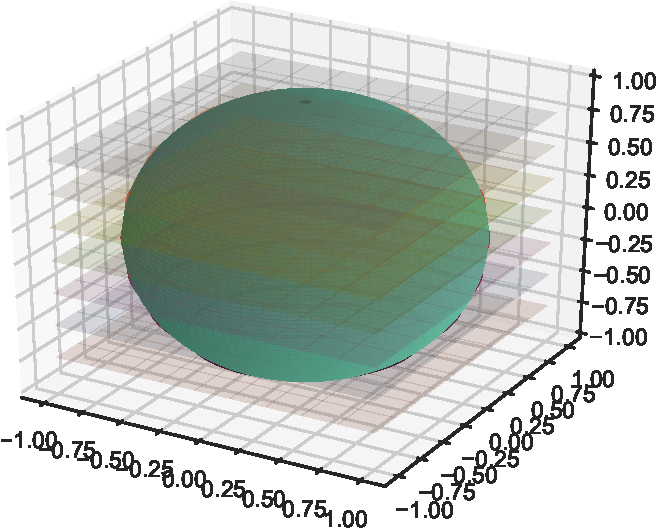
\includegraphics[scale=1.3]{../figures/sphere-crop.pdf}
    \label{fig:sphere}
\end{figure}

    \subsection{Marsaglia's Solution} \label{sec:2.1}
        \subsubsection{Intuition} \label{sec:2.1.1}
        Since the samples $x_1, \dots, x_n \sim \mathcal{N}(\mu, \sigma^2)$ we wish to generate are independent, we can write their joint density function as
        \begin{equation}
            \label{eqn:jointpdf}
            p(x_1, \dots, x_n) = \parens*{2\pi\sigma^2}^{-\sfrac{n}{2}}e^{-\sfrac{1}{2\sigma^2}\sum_{i = 1}^{n}\parens*{x_i - \mu}^2}.
        \end{equation}
        Thinking geometrically, we can envision the constraint in \autoref{eqn:mean} as defining a hyperplane in $\R^k$,
        and we can think of the constraint in \autoref{eqn:var} as defining the surface of a hypersphere in $\R^k$.
        Therefore, by generating $x_1, \dots, x_k$ satisfying the sample mean and sample variance conditions given by \autoref{eqn:mean} and \autoref{eqn:var} respectively,
        we are actually trying to sample points that lie on the intersection of an $k$-dimensional hyperplane and an $k$-dimensional hypersphere,
        which would be a ``circle" in $\R^k$ (actually a hypersphere in $k - 1$ dimensions).
        Let this intersection be $\mathcal{X} \subseteq \R^k$.
        We can now crucially note that the joint density function is constant on $\mathcal{X}$.
        Indeed, for all $\mathbf{x} = \parens*{x_1, \dots, x_k} \in \mathcal{X}$, we can observe
        \begin{align*}
            \sum_{i = 1}^{k}\parens*{x_i - \mu}^2 &= \sum_{i = 1}^{k}\parens*{x_i - \eta}^2 + 2(\eta - \mu)\sum_{i = 1}^{k}(x_i - \eta) + k(\eta - \mu)^2\\
            &= \sum_{i = 1}^{k}\parens*{x_i - \eta}^2 + k(\eta - \mu)^2\\
            &= k\delta^2 + k(\eta - \mu)^2,
        \end{align*}
        since $\sum_{i = 1}^{k}(x_i - \eta) = \parens*{\sum_{i = 1}^{k}x_i} - k\eta = k\eta - k\eta = 0$.
        Using this result, we can rewrite the density function in \autoref{eqn:jointpdf} as
        \begin{equation}
            \label{eqn:jointpdf+}
            p(x_1, \dots, x_k) = \parens*{2\pi\sigma^2}^{-\sfrac{k}{2}}e^{-\sfrac{1}{2\sigma^2}\parens*{k\delta^2 + k(\eta - \mu)^2}},
        \end{equation}
        which is independent of $x_1, \dots, x_k$ and only dependent on $\parens*{\mu, \sigma^2, \eta, \delta^2}$,
        allowing us to conclude that the joint density function is constant on $\mathcal{X}$.

        This important fact tells us that the probability distribution of $x_1, \dots x_k$
        conditional on satisfying the constraints $x_1, \dots, x_k \in \mathcal{X}$ is just the uniform distribution on $\mathcal{X}$.
        Therefore, in order to generate our desired samples $x_1, \dots, x_k$, we simply need to sample uniformly from the surface of a hypersphere in $\R^{k - 1}$.
        More precisely, we can generate $\mathbf{x} = (x_1, \dots, x_k) \in \mathcal{X}$ given a point $\mathbf{z} = (z_1, \dots, z_k)$
        on the surface of the $(k - 1)$-dimensional unit sphere by solving the linear system
        \begin{equation}
            \label{eqn:linearsystem}
            \mathbf{x} = \parens*{\sqrt{k}\delta}\mathbf{z}B + \eta\mathbf{v}
        \end{equation}
        where $\mathbf{v} = (1, \dots, 1) \in \R^k$ and $B \in R^{(k - 1) \times k}$ is a matrix satisfying $BB^T = I$ and $B\mathbf{v}^T = 0$.
        By noting that $\norm*{\mathbf{z}}^2 = \mathbf{z}\mathbf{z}^T = 1$,
        we can easily verify that the solution to \autoref{eqn:linearsystem}, with these choices of $\mathbf{v}$ and $B$, satisfies the constraints on our sample moments:
        \begin{equation*}
            \mathbf{x}\mathbf{v}^T = \sum_{i = 1}^{k}x_i = k\eta\\
        \end{equation*}
        \begin{equation*}
            \parens*{\mathbf{x} - \eta\mathbf{v}}\parens*{\mathbf{x} - \eta\mathbf{v}}^T = k\delta^2\parens*{\mathbf{z}BB^T\mathbf{z}^T}
            = k\delta^2\parens*{\mathbf{z}\mathbf{z}^T} = k\delta^2
        \end{equation*}
        Note that we have written our vectors above horizontally instead of vertically, so when computing inner products and matrix-vector products,
        our transposes are in different locations in order to remain consistent with the standard definitions of the operations.
        We now provide a pseudocode description of the algorithm.

        \subsubsection{Pseudocode} \label{sec:2.1.2}
        In this algorithm, we assume that the desired sample mean is a random variable $\eta \sim \mathcal{N}\parens*{\mu, \sfrac{\sigma^2}{k}}$
        and that the desired sample variance is also a random variable satisfying $\frac{(k - 1)\delta^2}{\sigma^2} \sim \chi_{k - 1}^2$.
        We generate $\epsilon_1, \dots, \epsilon_k \sim \mathcal{N}(0, 1)$ using the Beasley-Springer-Moro algorithm.
        \begin{algorithm}[H]
            \label{alg:marsaglia}
            \caption{\sc MarsagliaSample}
            \begin{algorithmic}
                \STATE {\bf Input:} Desired number of samples $k \in \N$
                \STATE {~~~~~~~~~~} i.i.d. samples $\epsilon_1, \dots, \epsilon_{k - 1} \sim \mathcal{N}(0, 1)$
                \STATE {~~~~~~~~~~} Sample mean $\eta \sim \mathcal{N}(\mu, \frac{\sigma^2}{k})$
                \STATE {~~~~~~~~~~} Sample variance $\delta^2$ satisfying $\frac{(k - 1)\delta^2}{\sigma^2} \sim \chi_{k - 1}^2$
                \STATE {\bf Output:} $x_1, \dots, x_k \sim \mathcal{N}(\mu, \sigma^2)$ with sample mean $\eta$ and sample variance $\delta^2$
                \STATE
                \STATE $\gamma = \sqrt{k}\delta$
                \STATE $s = \sum_{i = 1}^{k} \epsilon_i^2$
                \FOR{$i \in \set*{1, \dots, k}$}
                    $z_i = \epsilon_i\parens*{(k - i)(k - i + 1)s}^{-\sfrac{1}{2}}$
                \ENDFOR
                \STATE $x_1 = (1 - k) \gamma z_1 + \eta$
                \STATE $x_k = \gamma\sum_{i = 1}^{k - 1}z_i + \eta$
                \FOR{$i \in \set*{2, \dots, k-1}$}
                    $x_i = \gamma\parens*{\sum_{j = 1}^{i - 1}(j - k)z_j} + \eta$
                \ENDFOR
                \RETURN $x_1, \dots, x_k$
            \end{algorithmic}
        \end{algorithm}
        The above algorithm is only proven to produce an output with the desired properties if the
        sample mean $\eta$ and sample variance $\delta^2$ are {\it random variables} as described above. 
        Therefore, if we attempt to na\"ively use the algorithm with some deterministic values like $\eta = \mu$ and $\delta^2 = \sigma^2$, for example,
        we are not guaranteed to receive $x_1, \dots, x_k$ with the desired sample moments.

        To solve this problem, we generate $\eta$ using the Beasley-Springer-Moro algorithm,
        which implements a numerical version of the Inverse Transformation method for the Gaussian CDF.
        We then compute $\delta^2$ by first generating $\frac{(k - 1)\delta^2}{\sigma^2}$, which needs to have the $\chi^2$ distribution with $k - 1$ degrees of freedom.
        In order to sample from that distribution,
        we use the fact that the $L_2$ norm squared of $k - 1$ standard Normal variates is a $\chi^2$ variate with $k - 1$ degrees of freedom.
        Therefore, we generate $k - 1$ standard normal variates using the Beasley-Springer-Moro algorithm, and then compute their squared $L_2$ norm,
        multiply by $\sigma^2$ and then divide by $k - 1$ in order to obtain $\delta^2$.

\section{Antithetic Sampling} \label{sec:3}
Now that we know how to generate $x_1, \dots, x_k$ with given sample moments $\eta$ and $\delta^2$,
we want to know how to reduce the variance in the sampling using antithetic variates.
More precisely, given a set of $k$ independent samples $x_1, \dots, x_k \sim \mathcal{N}(\mu, \sigma^2)$,
we want to generate a new set of $k$ Gaussian samples $\tilde{x}_1, \dots, \tilde{x}_k$
such that the combined sample moments of the two sample sets still satisfy
$\frac{1}{2k}\sum_{i = 1}^{k}x_i + \tilde{x}_i = \eta$ and $\frac{1}{2k}\sum_{i = 1}^{k}\parens*{x_i - \mu}^2 + \parens*{\tilde{x}_i - \mu}^2 = \delta^2$.
This second set of samples is {\it antithetic} to the original sample set.

This essentially all comes down to how to choose new sample moments $\tilde{\eta}$ and $\tilde{\delta}^2$ in such a way that they are ``opposite" to $\eta$ and $\delta^2$,
which we can accomplish through a clever use of the Inverse Transformation method of generating variates.
Given a random variable $X$ with CDF $F_X$, we can obtain a random variable $Y = F_X(X)$ which is distributed uniformly on $[0, 1]$.
We can then generate an {\it intermediate antithetic} variate $\tilde{Y} = 1 - Y$ which is also distributed uniformly on $[0, 1]$.
Finally, we obtain a random variable {\it antithetic} to $X$ by computing $\tilde{X} = F_X^{-1}(\tilde{Y})$ using the inverse CDF.
Thus, we obtain $X$ and $\tilde{X}$ marginally distributed identically, but with non-zero correlation.

For our sample moments, if we let $F_\eta$ represent a Gaussian CDF and $F_\delta$ represent a Chi-squared CDf, we can derive $\tilde{\eta}$ and $\tilde{\delta^2}$ by computing
\begin{equation}
    \label{eqn:antimean}
    \tilde{\eta} = F_\eta^{-1}\parens*{1 - F_\eta(\eta)}
\end{equation}
\begin{equation}
    \label{eqn:antivar}
    \frac{(k - 1)\tilde{\delta}^2}{\sigma^2} = F_\delta^{-1}\parens*{1 - F_\delta\parens*{\frac{(k - 1)\delta^2}{\sigma^2}}}.
\end{equation}
Therefore, we can easily derive a pseudocode for generating antithetic variates.
However, the Gaussian and Chi-squared cumulative distribution functions are not generally easily invertible.
Since $\eta$ is normally distributed, computing the inverse CDF of $\eta$ to simplifies to
\begin{equation*}
    \tilde{\eta} = 2*\mu - \eta.
\end{equation*}
For the inverse Chi-squared CDF, we use a result given by \hyperref[ref:hawkins]{Hawkins and Wixley},
which was documented in a survey paper by \hyperref[ref:canal]{Canal} in $2005$.
This approach yields a closed form given by
\begin{equation*}
    \tilde{\lambda} = v\parens*{2\parens*{1 - \frac{3}{16v} - \frac{7}{512v^2} + \frac{231}{8192v^3}} - \parens*{\frac{\lambda}{v}}^\sfrac{1}{4}}^4
\end{equation*}
where $\lambda \sim \chi_v^2$ with $v = k - 1$ degrees of freedom.
The pseudocode is then as follows.

    \subsection{Pseudocode} \label{sec:3.1}
    \begin{algorithm}[H]
        \label{alg:antithetic}
        \caption{\sc AntitheticSample}
        \begin{algorithmic}
            \STATE {\bf Input:} i.i.d. samples $x_1, \dots, x_k \sim \mathcal{N}(\mu, \sigma^2)$
            \STATE {~~~~~~~~~~} Population mean and variance $\mu$ and $\sigma^2$
            \STATE {\bf Output:} $\tilde{x}_1, \dots, \tilde{x}_k \sim \mathcal{N}(\mu, \sigma^2)$ with sample mean $\tilde{\eta}$ and sample variance $\tilde{\delta}^2$
            \STATE
            \STATE $v = k - 1$
            \STATE $\eta = \frac{1}{k}\sum_{i = 1}^{k}x_i$
            \STATE $\delta^2 = \frac{1}{k}\sum_{i = 1}^{k}\parens*{x_i - \mu}^2$
            \STATE $\tilde{\eta} = 2\mu - \eta$
            \STATE $\lambda = \sfrac{v\delta^2}{\sigma^2}$
            \STATE $\tilde{\lambda} = v\parens*{2\parens*{1 - \frac{3}{16v} - \frac{7}{512v^2} + \frac{231}{8192v^3}} - \parens*{\frac{\lambda}{v}}^{\sfrac{1}{4}}}^4$
            \STATE $\tilde{\delta}^2 = \sfrac{\tilde{\lambda}\sigma^2}{v}$
            \STATE $\tilde{x}_1, \dots, \tilde{x}_k = \textsc{MarsagliaSample}(k, \tilde{\eta}, \tilde{\delta}^2)$
            \RETURN $\tilde{x}_1, \dots, \tilde{x}_k$
        \end{algorithmic}
    \end{algorithm}
\newpage
\section{Numerical Experiments} \label{sec:4}
To test how these algorithms work empirically, we compared the performance of \hyperref[alg:marsaglia]{Algorithm 1} to \hyperref[alg:antithetic]{Algorithm 2}
when tasked with sampling from a standard normal distribution using different numbers of samples $k$.
The algorithms are compared to the ``true" standard normal distribution, as given by the \texttt{norm.pdf()} function in SciPy's \texttt{stats} package.

The data sets labelled {\sc MarsagliaSample} are computed using $2k$ samples by using \hyperref[alg:marsaglia]{Algorithm 1} with $2k$ set as the number of desired samples.
The data sets labelled {\sc AntitheticSample} are computed by first generating $k$ samples using \hyperref[alg:marsaglia]{Algorithm 1},
and then using those as inputs to produce $k$ more samples from \hyperref[alg:antithetic]{Algorithm 2}.
In either case, the resulting graphs are generated by fitting a Gaussian curve to the raw data produced by the algorithms.
The \texttt{norm.pdf()} function was again used to fit those curves.
The results are visualized below.
\begin{figure}[H]
\centering
    \begin{minipage}{.49\textwidth}
        \centering
        \caption{$k = 8$ samples}
        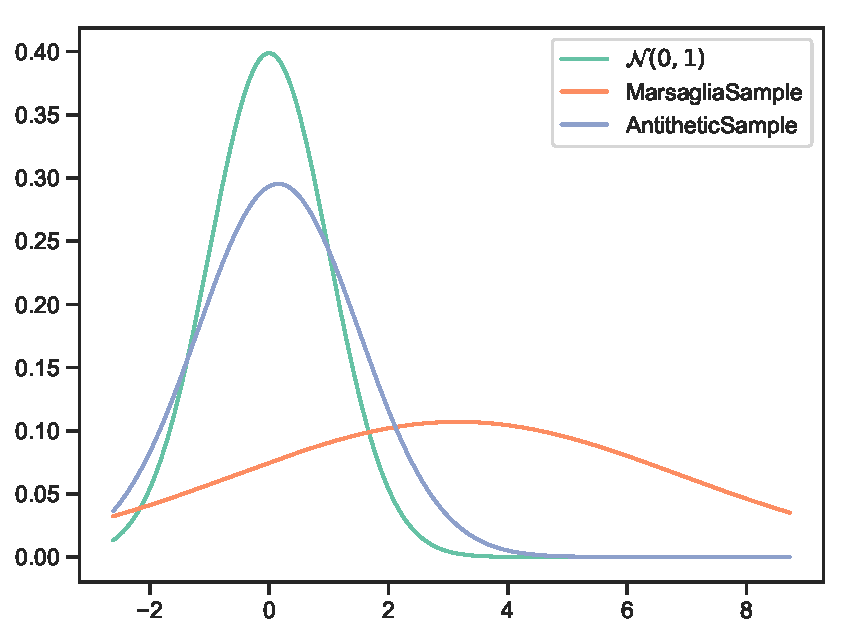
\includegraphics[scale=0.6]{../figures/normal-k8.pdf}
    \end{minipage}
    \begin{minipage}{.49\textwidth}
        \centering
        \caption{$k = 10$ samples}
        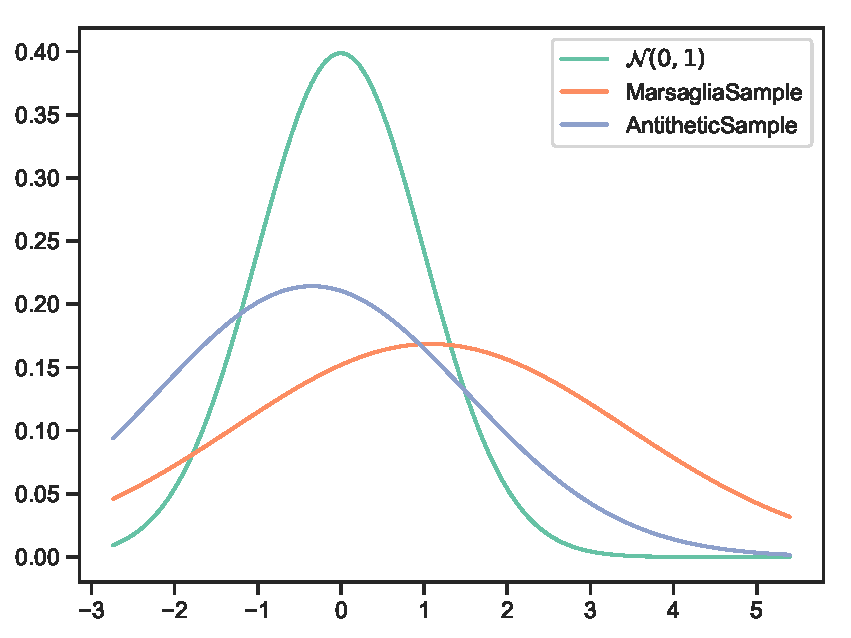
\includegraphics[scale=0.6]{../figures/normal-k10.pdf}
    \end{minipage}
    \begin{minipage}{\textwidth}
        \centering
        \caption{$k = 20$ samples}
        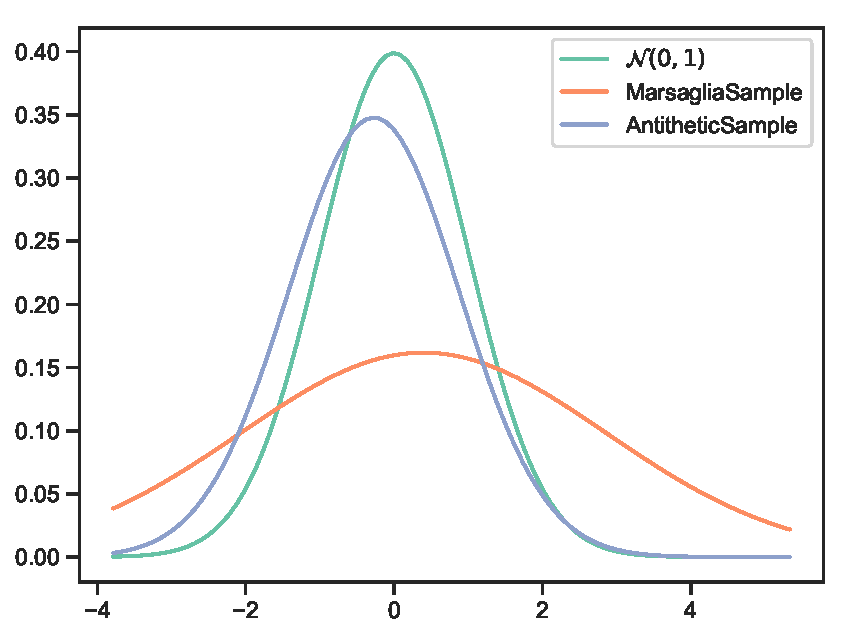
\includegraphics[scale=1]{../figures/normal-k20.pdf}
    \end{minipage}
\end{figure}

\section{Conclusion} \label{sec:5}
As we can see by the figures above, the antithetic approach of synthesizing the i.i.d. samples produced by \hyperref[alg:marsaglia]{Algorithm 1}
with the antithetic variates produced by \hyperref[alg:antithetic]{Algorithm 2} improves significantly upon the na\"ive approach that does not rely on antithetic variates.
Even with as few as $k = 8$ regular and $k = 8$ antithetic variates generated, we already obtain a fairly faithful approximation to the standard normal curve,
whereas the method which produces $k = 16$ variates without antithetic synthesis is clearly way off the mark.
The situation improves mildly for the non-antithetic method with $k = 40$ samples, but it is still heavily outperformed by the method
which synthesizes $k = 20$ regular and $k = 20$ antithetic samples.

\section*{References} \label{sec:ref}

\begin{itemize}
    \item \label{ref:marsaglia}
        G. Marsaglia and I. Good. C69. Generating a normal sample with given sample mean and variance.
        {\it Journal of Statistical Computation and Simulation}, 11 (1):71-74, 1980.
    \item \label{ref:canal}
        L. Canal. A normal approximation for the chi-square distribution. {\it Computational Statistics \& Data Analysis}, 48(4):803-808, 2005.
    \item \label{ref:hawkins}
        D. M. Hawkins and R. Wixley. A note on the transformation of chi-squared variables to normality. {\it The American Statistician}, 40(4):296-298, 1986.
\end{itemize}

\end{document}
